
\subsection{Selectors}

A \verb|Selector| is a class instance that should test whether a given tree node matches the rules defined by the \verb|Selector|. 
The \verb|Selectors| can be divided into three different categories.

The first category are logical \verb|Selectors|. They should represent logical operations. 
There are two \verb|Selectors| defined by default, \verb|AndSelector| and \verb|OrSelector|. 
Each takes a list of other selectors. The \verb|AndSelector| will only match tree nodes that match all passed \verb|Selectors|. 
The \verb|OrSelector| will match all tree nodes where at least one of the passed \verb|Selectors| matches the node.


The second category are data \verb|Selectors|. 
These selectors search for nodes based on the data they contain. 
They can match the name of a production, the alias of a production, the name of a lexer definition, and the value of a lexer token. 
The implemented selectors are \verb|AliasSelector|,\verb|ProductionSelector|,\verb|TokenSelector|,\verb|TokenValueSelector|. 
All of these take a string as a parameter and check the corresponding notes for that string.


The last category are structural \verb|Selectors|. 
These selectors search for nodes that have specific nodes in their children or parents.

The following example of an AST should illustrate the purpose of this category.

\begin{figure}[H]
    \centering
	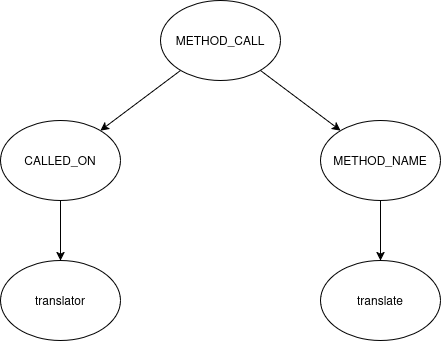
\includegraphics[scale=0.4]{"fig/selector_ast_example.png"}
    \caption{AST example for selectors}
\end{figure}

To search for all \verb|METHOD_CALL| nodes, that call translate on a translator object, we will want these types of selectors.

An example selector for this would be

\begin{lstlisting}[language=Java, caption=Selector example]
new AndSelector(
	new ProductionSelector("METHOD_CALL"),
	new HasImmediateChildSelector(
		new AndSelector(
			new ProductionSelector("CALLED_ON"),
			new HasImmediateChildSelector(
				new TokenValueSelector("translator")
			)
		)
	),
	new HasImmediateChildSelector(
		new AndSelector(
			new ProductionSelector("METHOD_NAME"),
			new HasImmediateChildSelector(
				new TokenValueSelector("translate")
			)
		)
	)
)
\end{lstlisting}

By calling the \verb|query| method on the root node of the AST, we get all the \verb|METHOD_CALL| nodes in the AST that match those conditions.
